\chapter{Algorithms Complexity}

\section{What is an algorithm?}

An algorithm is a sequence of steps to solve a problem. It is a finite set 
of instructions that, when followed, accomplish a particular task. An 
algorithm is a tool for solving a well-specified computational problem. 
It is a recipe for computation, a sequence of steps that specifies how to 
solve a problem.\\

The branch of computer science that studies algorithms is called
\textbf{algorithm analysis} or \textbf{computational complexity}. It is
concerned with the theoretical study of computer-program performance and
resource usage.\\

Why do we need to study algorithms in a formal way? Algorithm analysis helps us
to understand the performance of an algorithm. It provides a way to compare
different algorithms for the same problem. It also provides a way to understand
the limitations and scalability of a program.

\section{Asymptotic Notation}

The performance of an algorithm is measured in terms of the input size. The
input size is the number of bits required to represent the input. The
performance of an algorithm is also measured in terms of the number of
operations performed by the algorithm. The number of operations performed by an
algorithm is a function of the input size.\\

To analyze the performance of an algorithm, we need to study the growth rate of
this function. For this purpose, we use the \textbf{asymptotic notation}. The
asymptotic notation is a mathematical notation that describes the limiting
behavior of a function as the input size approaches infinity. We will define
three asymptotic notations: big-O notation, big-$\Omega$ notation, and
big-$\Theta$ notation.

\subsection{Big-O Notation}

The big-O notation is used to describe the upper bound of a function. Formally,
we say that $f(n)$ is $O(g(n))$ if there exist positive constants $c$ and $n_0$
such that:

\begin{equation}
    0 \leq f(n) \leq c \cdot g(n) \quad \forall n \geq n_0
\end{equation}

In other words, $f(n)$ is $O(g(n))$ if there exists a constant $c$ such that
$f(n)$ is bounded above by $c \cdot g(n)$ for all $n$ greater than some
threshold $n_0$.\\

For example, the function $f(n) = 3n^2 + 2n + 1$ is $O(n^2)$ because $3n^2 + 2n
+ 1 \leq 6n^2$ for all $n \geq 1$. In this case, $c = 6$ and $n_0 = 1$.\\

The big-O notation is used to describe the worst-case performance of an
algorithm. It provides an upper bound on the number of operations performed by
the algorithm. The main classes of functions used in the big-O notation are:

\begin{itemize}
    \item Constant functions: $O(1)$
    \item Logarithmic functions: $O(\log n)$
    \item Linear functions: $O(n)$
    \item Linearithmic functions: $O(n \log n)$
    \item Quadratic functions: $O(n^2)$
    \item Cubic functions: $O(n^3)$
    \item Exponential functions: $O(2^n)$
\end{itemize}

\subsection{Big-$\Omega$ Notation}

The big-$\Omega$ notation is used to describe the lower bound of a function.
Formally, we say that $f(n)$ is $\Omega(g(n))$ if there exist positive constants
$c$ and $n_0$ such that:

\begin{equation}
    0 \leq c \cdot g(n) \leq f(n) \quad \forall n \geq n_0
\end{equation}

In other words, $f(n)$ is $\Omega(g(n))$ if there exists a constant $c$ such
that $f(n)$ is bounded below by $c \cdot g(n)$ for all $n$ greater than some
threshold $n_0$.\\

For example, the function $f(n) = 3n^2 + 2n + 1$ is $\Omega(n^2)$ because $3n^2
+ 2n + 1 \geq n^2$ for all $n \geq 1$. In this case, $c = 1$ and $n_0 = 1$.\\

The big-$\Omega$ notation is used to describe the best-case performance of an
algorithm. It provides a lower bound on the number of operations performed by
the algorithm. The classes of functions used in the big-$\Omega$ notation are
the same as those used in the big-O notation.

\subsection{Big-$\Theta$ Notation}

The big-$\Theta$ notation is used to describe the tight bound of a function.
Formally, we say that $f(n)$ is $\Theta(g(n))$ if there exist positive constants
$c_1$, $c_2$, and $n_0$ such that:

\begin{equation}
    0 \leq c_1 \cdot g(n) \leq f(n) \leq c_2 \cdot g(n) \quad \forall n \geq n_0
\end{equation}

In other words, $f(n)$ is $\Theta(g(n))$ if there exist constants $c_1$ and
$c_2$ such that $f(n)$ is bounded above and below by $c_1 \cdot g(n)$ and $c_2
\cdot g(n)$, respectively, for all $n$ greater than some threshold $n_0$.\\

For example, the function $f(n) = 3n^2 + 2n + 1$ is $\Theta(n^2)$ because $n^2
\leq 3n^2 + 2n + 1 \leq 6n^2$ for all $n \geq 1$. In this case, $c_1 = 1$, $c_2
= 6$, and $n_0 = 1$.\\

The big-$\Theta$ notation is used to describe the average-case performance of
an algorithm. It provides a tight bound on the number of operations performed by
the algorithm. It is useful when we want to analyze the behavior of an algorithm
in a more precise way, although it is more difficult to determine. The classes of 
functions used in the big-$\Theta$ notation are the same as those used in the 
big-O notation.

\section{Sorting Algorithms}

Sorting is the process of arranging a list of elements in a specific order. The
most common orders are ascending and descending. Sorting is a fundamental
operation in computer science. It is used in many applications, such as
databases, search engines, and operating systems. There are many sorting
algorithms, each with its own advantages and disadvantages. In this section, we
will study some of the most popular sorting algorithms.

\subsection{Selection Sort}

Selection sort is a simple sorting algorithm that works by repeatedly selecting
the smallest (or largest) element from the unsorted part of the list and moving
it to the sorted part of the list. It is considered the naive sorting algorithm
because it is easy to implement and understand.\\

Its implementation is as follows:

\begin{lstlisting}[language=C++]
void selection_sort(int arr[], int n) {
    for (int i = 0; i < n - 1; i++) {
        int min_index = i;
        for (int j = i + 1; j < n; j++) {
            if (arr[j] < arr[min_index]) {
                min_index = j;
            }
        }
        swap(arr[i], arr[min_index]);
    }
}
\end{lstlisting}

The time complexity of selection sort is $O(n^2)$ in the worst-case and
average-case scenarios. The best-case time complexity is also $O(n^2)$ because
the algorithm always performs $n$ swaps, even if the list is already sorted.

\subsection{Insertion Sort}

Insertion sort is a simple sorting algorithm that works by repeatedly inserting
an element from the unsorted part of the list into its correct position in the
sorted part of the list. Its implementation is as follows:

\begin{lstlisting}[language=C++]
void insertion_sort(int arr[], int n) {
    for (int i = 1; i < n; i++) {
        int key = arr[i];
        int j = i - 1;
        while (j >= 0 && arr[j] > key) {
            arr[j + 1] = arr[j];
            j--;
        }
        arr[j + 1] = key;
    }
}
\end{lstlisting}

The time complexity of insertion sort is $O(n^2)$ in the worst-case scenario,
$O(n)$ in the best-case scenario, and $O(n^2)$ in the average-case scenario.
The best-case time complexity is $O(n)$ because the algorithm performs $n - 1$
comparisons and no swaps when the list is already sorted.

\subsection{Merge Sort}

Merge sort is a divide-and-conquer sorting algorithm that works by dividing the
list into two halves, sorting each half recursively, and then merging the two
sorted halves. Its pseudocode is as follows:

\begin{algorithm}[H]
    \caption{Merge Sort}
    \begin{algorithmic}[1]
        \Function{MergeSort}{$arr[], l, r$}
            \If{$l < r$}
                \State $m \gets (l + r) / 2$
                \State \Call{MergeSort}{$arr, l, m$}
                \State \Call{MergeSort}{$arr, m + 1, r$}
                \State \Call{Merge}{$arr, l, m, r$}
            \EndIf
        \EndFunction
    \end{algorithmic}
\end{algorithm}

The \texttt{MERGE} function merges two sorted subarrays into a single sorted array. 
Its main steps are:

\begin{enumerate}
    \item Compare the first element of the left subarray with the first element of the 
    right subarray.
    \item If the first element of the left subarray is smaller, copy it to the output 
    array
    \item Otherwise, copy the first element of the right subarray to the output array
    \item Repeat the process until all elements are copied to the output array
\end{enumerate}

The time complexity of merge sort is $O(n \log n)$ in all scenarios. This is because 
the operation of recursively dividing the list into two halves reduces the size of 
the problem by a factor of 2 in each step. The amout of times we can divide the list 
by 2 is $\log_2 n$, where $n$ is the size of the list. The merge operation has a time 
complexity of $O(n)$, where $n$ is the size of the list. Therefore, the total time 
complexity of merge sort is $O(n \log n)$.\\

The divide-and-conquer paradigm usually results in algorithms with a time complexity
with a logarithmic factor. 

\section{Big-O complexity chart}

The following chart shows the comparison of the most common time complexities in
computer science:

\begin{figure}[H]
    \centering
    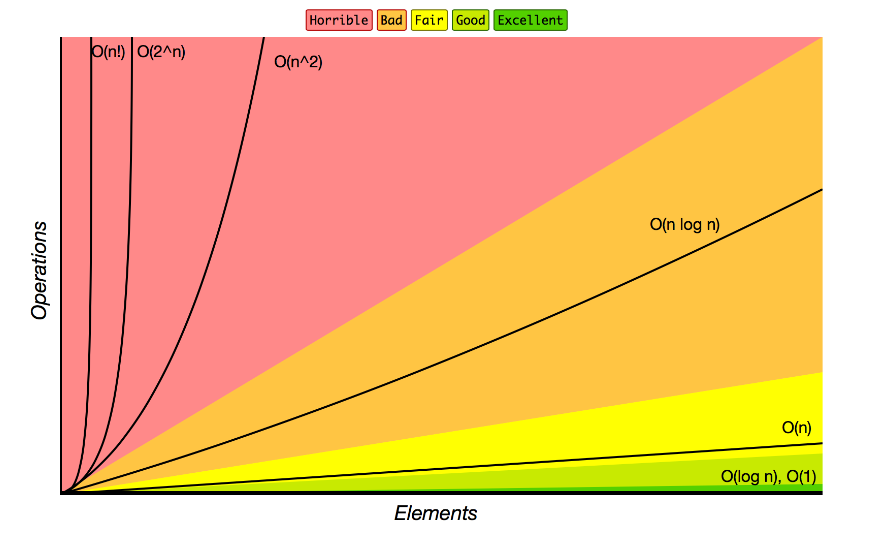
\includegraphics[width=0.8\textwidth]{figures/image_big-o.png}
    \caption{Big-O complexity chart}
    \label{fig:big-o}
\end{figure}

